\documentclass[sigconf,natbib=false,10pt]{acmart}

%%
%% \BibTeX command to typeset BibTeX logo in the docs
\AtBeginDocument{%
	\providecommand\BibTeX{{%
			Bib\TeX}}}

%% Rights management information.  This information is sent to you
%% when you complete the rights form.  These commands have SAMPLE
%% values in them; it is your responsibility as an author to replace
%% the commands and values with those provided to you when you
%% complete the rights form.
%\setcopyright{acmlicensed}
%\copyrightyear{2018}
%\acmYear{2018}
%\acmDOI{XXXXXXX.XXXXXXX}

%% Bibliography style
\RequirePackage[datamodel=acmdatamodel,style=acmnumeric]{biblatex}

%% Declare bibliography sources
\addbibresource{reference.bib}

%%
%% end of the preamble, start of the body of the document source.
\begin{document}
	
	%%
	%% The "title" command has an optional parameter,
	%% allowing the author to define a "short title" to be used in page headers.
	\title{Assistant Tools and Accessibility Features for Blind People Playing Visual-Centric Digital Games}
	
	\author{Marco Prescher}
	%\authornote{This is a author note!}
	\affiliation{%
		\institution{FHV University of Applied Sciences}
		\streetaddress{Hochschulstraße 1}
		\city{Dornbirn}
		\state{Vorarlberg}
		\country{Austria}}
		\postcode{6850}
	\email{marco.prescher@students.fhv.at}
	
	%%
	%% By default, the full list of authors will be used in the page
	%% headers. Often, this list is too long, and will overlap
	%% other information printed in the page headers. This command allows
	%% the author to define a more concise list
	%% of authors' names for this purpose.
	\renewcommand{\shortauthors}{Marco Prescher}
	
	%%
	%% The abstract is a short summary of the work to be presented in the
	%% article.
	%TODO
	\begin{abstract}
		Lorem ipsum dolor sit amet, consectetur adipiscing elit. Morbi
		malesuada, quam in pulvinar varius, metus nunc fermentum urna, id
		sollicitudin purus odio sit amet enim. Aliquam ullamcorper eu ipsum
		vel mollis. Curabitur quis dictum nisl. Phasellus vel semper risus, et
		lacinia dolor. Integer ultricies commodo sem nec semper.
	\end{abstract}
	
	\ccsdesc[500]{Applied computing~Computer games}
	\ccsdesc[500]{Human-centered computing~Accessibility}
	\ccsdesc[500]{Human computer interaction (HCI)}
	
	%%
	%% Keywords. The author(s) should pick words that accurately describe
	%% the work being presented. Separate the keywords with commas.
	\keywords{blind, accessibility, gaming, digital games, navigation, tools, AI}
	
	%\received{20 February 2007}
	%\received[revised]{12 March 2009}
	%\received[accepted]{5 June 2009}
	
	%%
	%% This command processes the author and affiliation and title
	%% information and builds the first part of the formatted document.
	\maketitle
	
	\section{Introduction} \label{sec:introduction}
	Today's accessible games for blind people are mainly games which are directly developed for them (\textcite{goncalves_my_2023}).
	While these games are enjoyable, mainstream games are a serious challenge for blind people because they consist of complex environments, mechanics and interactions with \emph{Non-Player Character} (NPC) players or even real players in \emph{Player versus player} (PvP) games.
	
	Implementing accessibility features is much needed in digital games to ensure that everyone, including people with disabilities can enjoy gaming.
	However, game developers in general face various problems in the process of developing games, some of them are:
	
	\begin{itemize}
		\setlength\itemsep{0.5em}
		\item Diverse Needs
		\item Technical Challenges
		\item Design Compromises
		\item Standardization
	\end{itemize}
	
	So, the main idea of this paper is to give a broad insight of \emph{Universally Accessible Game Design} (UAGD) which addresses the previously mentioned developing problems.
	Additionally, this study explores different and innovative accessibility features and tools, including haptic feedback and its ways to improve game experience which is a major technical challenge.
	
	This raises following relevant research questions (RQ) that contribute to blind people playing visual-centric digital games:
	
	\begin{itemize}
		\setlength\itemsep{0.5em}
		\item RQ1: How can UAGD improve the development of games with regard to accessibility? (\autoref{subsec:uagd})
		\item RQ2: In what ways can haptic feedback enhancements improve the game experience for blind players? (\autoref{subsec:assistiveHapticFeedback})
		\item RQ3: Which innovative accessibility features and tools can enhance the gaming experience for blind players? (\autoref{subsec:improvements})
	\end{itemize}

	\subsection{Motivation}
	One big step forward making mainstream games more accessible for blind people was the game \emph{The Last of Us Part II} (TLOU2) \cite{playstation_last_2020, playstation_last_2020-1}. 
	According to \textcite{leite_extended_2021} the game company \emph{Naughty Dog} implemented more than 60 accessibility features and is considered as the most accessible game ever produced (See \autoref{fig:tlou-accessibility-presets}).
	
	\begin{figure*}[ht]
		\centering
		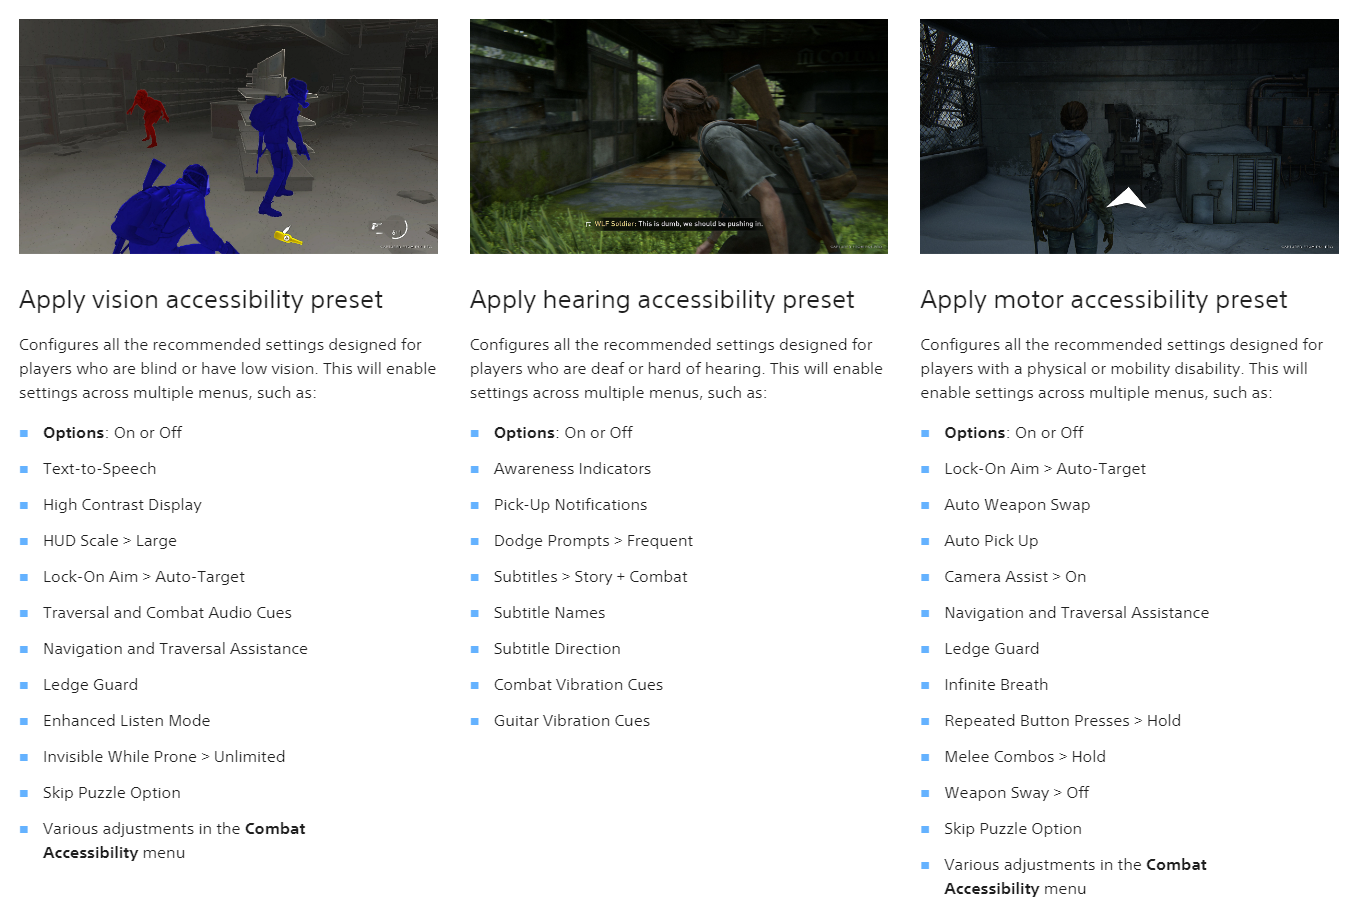
\includegraphics[scale=0.6,width=\textwidth]{assets/tlou-accessibility-presets.png}
		\caption{Accessibility presets in TLOU2 (Source: \textcite{playstation_last_2020-1})}
		\label{fig:tlou-accessibility-presets}
	\end{figure*}

	Additionally, \textcite{dale_last_2024} described that the game can be played all the way through with audio cues and navigation aids.
	It includes preset accessibility options for common disabilities like hearing or vision impairments. 
	It also introduces accessibility menus when the game is first started, making it easier for players with disabilities to adjust settings.
	To top that, \emph{Naughty Dog} released a remastered version of TLOU2 in 2024 with a reworked \emph{Cinematic Audio Descriptions} feature \cite{playstation_last_2024}.
	
	In the past, video games were not designed with accessibility mind, which resulted in bad gaming experience for people with disabilities. 
	However, over time, game companies started to develop and include accessibility features in their games which significantly improved the game experience for disabled players.
	
	However, there are still many games which were not developed in a way that everyone can play it.
	With focus on blind players, this paper aims to find a way to help the development cycle of games as well as exploring existing accessibly features and ways to enhance them.
	
	\section{The Problem} \label{sec:theProblem}
	Blind players encounter many different barriers when playing visual-centric digital games which often rely mainly on graphical interfaces and visual cues. 
	Additionally, games have different perspectives such as top-down, first-person, and third-person views, where all three views give the player unique challenges in navigating within game environments, understanding game objectives and interacting with in-game elements like players or objects.
	
	Popular games, such as \emph{The Legend of Zelda} rely mainly on visuals.
	For blind players, this is obviously a big problem because they miss a lot of important information on how to complete tasks or what is happening around them.
	
	As \textcite{goncalves_my_2023} states, players express feelings of frustration, telling their viewers the need for more and better accessibility features, so that everyone including blind players can have a great game experience.
	
	Building on that, the authors of \textcite{goncalves_my_2023} have categorized seven themes and identified unresolved barriers (see \autoref{fig:seven-themes}) which still represent a great challenge for both players and developers.
	
	\begin{figure*}[ht]
		\centering
		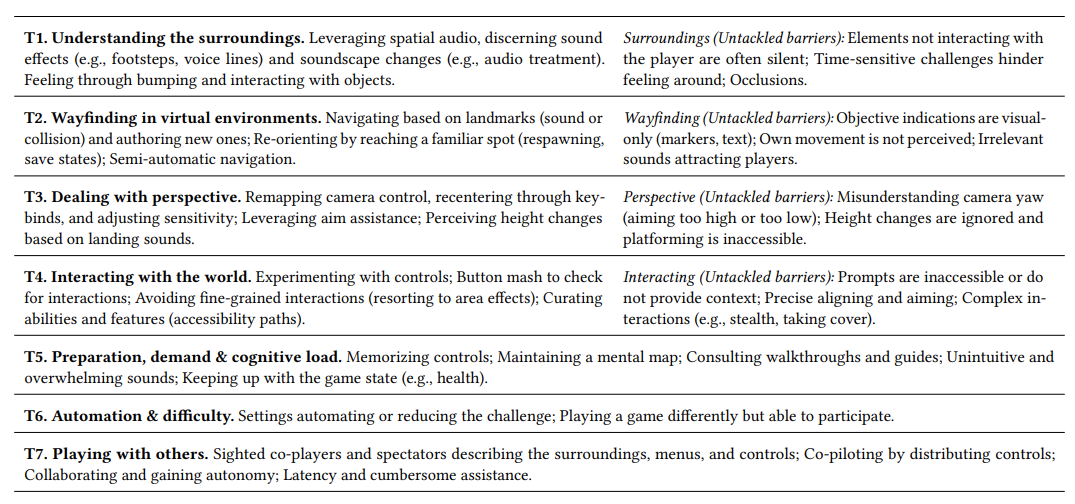
\includegraphics[scale=0.6,width=\textwidth]{assets/seven-themes.png}
		\caption{Seven themes and respective unresolved barriers (Source: \textcite{goncalves_my_2023})}
		\label{fig:seven-themes}
	\end{figure*}

	\autoref{fig:seven-themes} gives a great overview what accessibility features are still missing and in which direction the gaming industry should focus.
	
	\section{My Idea} \label{sec:myIdea}
	The gaming industry came a long way from no accessibility features and assistant tools at all to implementing more than 60 accessibility features in one game \cite{playstation_last_2020}.
	According to research papers \cite{goncalves_my_2023, grammenos_designing_2009, grammenos_game_2008, araujo_mobile_2017} some of the most important accessibility features for blind people in visual-centric games include:
	
	\begin{itemize}
		\setlength\itemsep{0.5em}
		\item Audio Cues and Descriptions
		\item \emph{Text-to-Speech} (TTS) and Voiceover
		\item Navigation Aids and Wayfinding Tools
		\item Comprehensive Audio Design
		\item Customizable Controls and Inputs
		\item Tactile Feedback and Controller Design
	\end{itemize}
    
    Some of these have already been implemented to a certain extent in some games, but as \autoref{fig:seven-themes} notes, there are still problems.
    Especially when it comes to the environment, pathfinding, perspective and interacting with the world, blind players face major challenges, which according to \textcite{goncalves_my_2023} could mean they stop playing these games because they simply can not find the right way to play.
    
    To address the environment and pathfinding problems, one new technology was introduced in 2018 by \textcite{andrade_echo-house_2018} to use echolocation to explore a virtual environment which could drastically improve navigation in it.
    As for perspective (camera) and interacting with the world, hardware solutions like haptic feedback or \emph{Artificial Intelligence} (AI) tools could be a solution when developed and integrated further.
    Whereas the haptic feedback \cite{bello_haptics_2016} of for example PS5-Controllers \cite{akyaman_anticipated_2021, chen_gamepad_2024} could indicate the environment they are walking on by adjusting the vibrations.
    
    The goal is to find an answer to the research question above by researching the field of UAGD, how to use haptic feedback to improve accessibility features and to find new ways to enhance existing accessibility features and tool in combination with AI.
    Therefore, game developers should use the UAGD as a guide and ensure that all important accessibility features listed above are included in their games.
    
    The following section provides a deeper insight into related work that has contributed to the understanding of the importance of accessibility in visual-centric digital games.
	
	\section{Related Work} \label{sec:relatedWork}
	As digital games continuous to evolve making them more complex to play, accessibility becomes increasingly more important.
	This section provides a deeper insight into related work that has contributed to the understanding of the importance of accessibility in visual-centric digital games.
	
	\subsection{Themes of accessibility}
	The paper \textcite{goncalves_my_2023} explores the strategies blind players use to play visual-centric mainstream games.
	It analyzes over 70 hours of YouTube content from blind players to identify the strategies and methods they use to navigate and interact within games environments.
	
	The study highlights that blind players often rely on audio cues to understand and navigate within game environments.
	They use repetitive actions like bumping into a wall to create a mental map of the environment.
	Players also try to create landmarks by interacting with the game world, for example, by leaving enemies behind to know in which area they are at the moment.
	This approach helps to navigate within game environments but also scare of new blind players due to frustration if the player become disorientated.
	
	The result of their findings are seven themes focusing on describing strategies blind players created and adopted: (See \autoref{fig:seven-themes})
	
	\begin{itemize}
		\setlength\itemsep{0.5em}
		\item Understanding the surroundings
		\item Wayfnding in virtual environments
		\item Dealing with perspective
		\item Interacting with the world
		\item Preparation, demand and cognitive load
		\item Automation and difficulty
		\item Playing with others
	\end{itemize}

	Additionally, \autoref{fig:seven-themes} shows us the existing barriers mainstream games have.
	
	The paper also acknowledges the efforts of some game developers to make new and existing games more accessible to blind players.
	This approach by developers is essential for reducing the accessibility gap in the upcoming years of game development.
	
	\subsection{Inaccessibility in Games}
	In 2008 \textcite{grammenos_game_2008} developed a game called \emph{Game Over!}, which is the first universally inaccessible game, created as an educational tool to teach game developers about accessibility guidelines.
	This approach aimed to raise awareness and motivate game developers to make their games accessible for everyone.
	
	The developed game \emph{Game Over!} has 21 levels implemented, each one violating a specific game accessibility guideline to frustrate but also educate by directly showing the developer what impact their design decisions have. 
	Some of the guidelines are:
	
	\begin{itemize}
		\setlength\itemsep{0.5em}
		\item Require complex key combinations
		\item Rapidly changing control schemes
		\item Presenting information in inaccessible formats
	\end{itemize}

 	Collected feedback from developers and players through surveys and public discussions indicate that the game raises awareness and educates about accessibility as intended.
 	It also suggested for the game to include direct access to additional information about each violated guideline, such as how specific accessibility can improve the game experience for disabled players.
 	
 	The feedback also highlighted to add more levels to cover a wider range of accessibility guidelines which would add the potential to adapt the concept and further improve it as well as to highlight the importance of game design in digital games.
	
	\subsection{Navigate a virtual environment using echolocation}
	In 2018 \textcite{andrade_echo-house_2018} investigates the use of echolocation in a game environment to help blind players to navigate in them.
	This approach aimed to investigate whether it is possible to create a \emph{virtual environment} (VE) where players can simulate echolocation to navigate and understand complex scenes within that VE.
	
	Therefore, they developed a VE with Unity 5.6 and the SteamAudio plug-in.
	This VE basically represents a three level house called \emph{Echo-House}, where users can navigate using sounds such as mouth-clicks, claps and footsteps, which generate echoes to receive information about the environment.
	Each level had a goal players needed to reach to get to the next level of the house (See \autoref{fig:echo-house-layout}).
	
	\begin{figure}[ht]
		\centering
		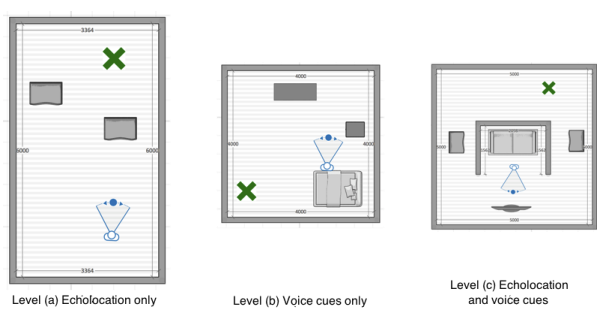
\includegraphics[scale=0.5]{assets/echo-house-layout.png}
		\caption{Layout of the three levels (Source: \textcite{andrade_echo-house_2018})}
		\label{fig:echo-house-layout}
	\end{figure}

	The evaluation consists of a 45-minute playing session and a interview.
	They found out that the echolocation provided the player with an improved sense of space within the VE.
	However, challenges in orientation and mobility were still present which indicates the need of further support.
	
	The paper highlighted the limitation of the study such as the small sample size and the need for further research to validate their findings.
	Nevertheless, this work provides an important insight into the possibilities of using echolocation to help blind players.
	
	\section{The Details} \label{sec:theDetails}
	In this section, we delve into enhancing accessibility in digital games for blind players.
	Firstly, we aim to explore previously mentioned developing problems in \autoref{sec:introduction}, from diverse needs and technical challenges followed by design compromises and standardization efforts.
	Secondly, we explore various types of feedback which are essential in enhancing of accessibility in digital games and focus on haptic feedback as well as further possibilities to use that to improve the experience in digital games for blind players.
	Lastly, we propose enhancements of already existing accessibility features and tools.
	
	\subsection{Universally Accessible Game Design} \label{subsec:uagd}
	In recent years, the awareness of accessible game design has been growing tremendously.
	According to \emph{World Health Organization} \cite{world_health_organization_international_2004}, one out of ten persons has disabilities which often results in limitations in hearing, memory, vision or motor functions.
	
	\subsubsection{Addressing Diverse Needs}
	Digital games are getting more demanding in terms of limitations and this is where UAGD comes into play.
	Through the implementation of UAGD, players with diverse needs can benefit from features such as support for alternative input devices, including switches, eye-tracking systems, and mouth-operated controllers, which as a result can drastically enhance the game experience.
	By implementing these features, UAGD ensures that games are accessible to players with various disabilities, ensuring that games are enjoyable for a wider audience.
	
	\subsubsection{Technical Challenges}
	Implementing UAGD presents several technical challenges including compatibility with different hardware and the scalability of accessibility features.
	By using a user-centered approach, as presented by \textcite{grammenos_unified_2007}, developers can integrate accessibility into the game development cycle and ensure that technical challenges are considered from the beginning of the project.
	The basic steps are (See \autoref{fig:universal-game-design-approach}):
	
	\begin{itemize}
		\setlength\itemsep{0.5em}
		\item Abstract task-based game design
		\item Polymorphic specialization with design alternatives
		\item Appropriateness analysis for the design alternatives
		\item Compatibility analysis among design alternatives
		\item Prototyping
		\item Usability and accessibility evaluation
	\end{itemize}
	
	An elaboration of these steps is provided in \textcite{grammenos_unified_2007}
	
	\begin{figure}[ht]
		\centering
		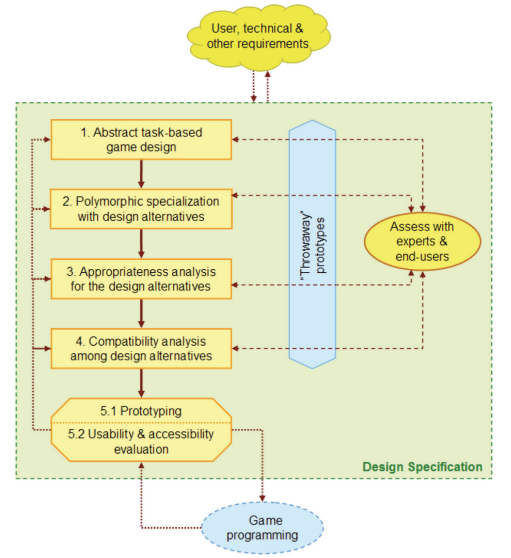
\includegraphics[scale=0.5]{assets/universal-game-design-approach.png}
		\caption{Applying UAGD (Source: \textcite{grammenos_unified_2007})}
		\label{fig:universal-game-design-approach}
	\end{figure}
	
	\subsubsection{Design Compromises}
	UAGD encourages developers to rethink design approaches, so that all players can enjoy the game they are developing.
	This includes reimagining game mechanics, levels, and interfaces to ensure everyone gets the best game experience without destroying the games core idea.
	The key here is to create games which are challenging and fun to play for all the players, regardless of their abilities.
	
	\subsubsection{Standardization Efforts}
	An important aspect of UAGD is to push towards standardizing accessibility features in all games.
	To achieve that, common guidelines and best practices are needed, so that the gaming industry can create a more standardized approach to accessibility, making it easier for developers to implement these.
	One key aspect here is to share those approaches and ideas with the software community as well as make the implementations open source.
	
	In summary, UAGD is not just about making games playable for players with disabilities.
	It should redefine how a game is developed and designed, so that the needs of all players are satisfied.
	
	\subsection{Assistive haptic feedback} \label{subsec:assistiveHapticFeedback}
	Assistive haptic feedback gets increasingly more important, especially in the gaming industry \cite{kuber_towards_2007}.
	In this section we delve into innovative approaches to enhance the gaming experience for blind player through tactile technologies.
	First we will give an overview of sensory perception which consists of visual (sight), haptic (tactile), and aural (hearing) as shown in \autoref{fig:sensory-perception}.
	Then we will explore different possibilities to enhance game experience with haptic feedback.
	
	\begin{figure}[ht]
		\centering
		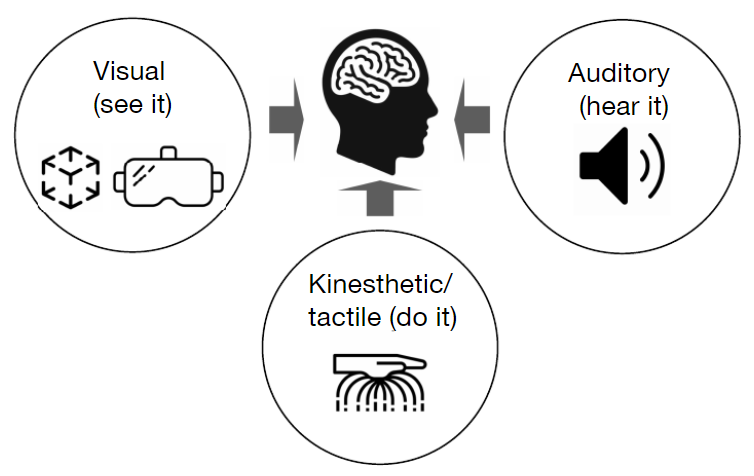
\includegraphics[scale=0.4]{assets/sensory-perception.png}
		\caption{Sensory perception (Source: \textcite{sanfilippo_perspective_2022})}
		\label{fig:sensory-perception}
	\end{figure}
	
	\subsubsection{Sensory Perception in Gaming for Blind Players}
	Gaming experience for blind people primarily rely on non-visual sensory to navigated and interact within the game environment.
	Visual perception which the player mainly get though sight, is often the primary interaction in most games.
	However, for blind player, haptic and aural senses are the key.,
	
	Haptic feedback is the sense of touch providing a physical response by vibration to the player \cite{chen_gamepad_2024, kuber_towards_2007, bello_haptics_2016}, which represent various action in a game like drawing a bow or shooting a weapon.
	For example, a haptic glove could simulate the sensation of raindrops falling on a player's hand or the resistance encountered when pushing against an in-game object.
	
	Aural feedback, in the other hand, provides sound to transfer information.
	For example, the sound of footsteps can indicate that an ally or enemy is approaching, while footstep sounds changes indicate a transition from one area to another, such as moving from a city street into a quiet building.
	
	\subsubsection{Enhancing Gaming Experience through Assistive Haptic Feedback}
	Assistive haptic feedback helps blind players feel and interact with game worlds through touch.
	This form of feedback offers a new dimension of immersion and accessibility.
	For example, vibration can be designed in a way that they give information to the player by providing them with different vibration patterns on various surfaces such as uneven roads or a sandy beach.
	By doing that, players receive a sense of location and movement within the game environment.
	
	Beyond that, advanced haptic technologies like shape-changing interfaces or dynamic touch surfaces \cite{rasmussen_shape-changing_2012} can simulate more complex interactions.
	These could include the sensation of touching sand or feel the resistance when drawing a bowstring by using a haptic glove mentioned previously.
	This feedback technology could also help in navigating within a game environment where pulses could indicate the direction a player has to go.
	This not only makes games more accessible to blind players but also increase the dimension of immersion for all players.
	
	Considering the impact of standardizing this technology as a guideline within UAGD, making it a straightforward implementation for developers would help the game industry tremendously in terms of accessibility.
	
	\subsection{Ways to improve existing accessibility features and tools} \label{subsec:improvements}
	In this section we explore strategies to improve accessibility for blind players.
	We are focusing us here on two promising advanced technology ideas:
	
	\begin{itemize}
		\setlength\itemsep{0.5em}
		\item AI-Enhanced Testing and Audio Descriptions
		\item Combining AI with echolocation techniques
	\end{itemize}

	\subsubsection{AI-Enhanced Testing and Audio Descriptions}
	By implementing AI into the cycle of game development, we could significantly improve the accessibility for blind players by integration AI into the testing phase of the game.
	After collecting enough data about accessibility, the AI could automate the testing phase, identifying accessibility issues or UAGD guideline violations which are not immediately visible for the developer.
	This would ensure that games are designed the right way from the start.
	
	Additionally, by letting the AI collect data during game play tests, it could generate real-time audio descriptions of game environments and action which could improve the gaming experience for blind players.
	The generated descriptions can then customize for the needs of individual players.
	
	To implement this method, additional research and testing are required.
	This approach would greatly help developers in designing future games.
	
	\subsubsection{Combining AI with Echolocation for Navigation}
	Combining AI with echolocation technology could assist blind players in navigating within game environments.
	The AI could interpret the echolocation signals which could be combined with haptic or aural feedback, helping players understand their environment.
	For example, a glove or body armor as haptic feedback devices could receive the signals, process them to create a detailed map of the surroundings which provides the player with a much better understanding what is happening.
	
	For this technology to be fully realized, further research like \textcite{andrade_echo-house_2018} is required.
	This approach is promising for not only enhancing the experience for blind but all players.
	
	\section{Conclusions and Further Work}
	This paper addressed the challenge of enhancing accessibility features in digital games for blind players.
	Our proposed solution is centered around \emph{Universally Accessible Game Design} (UAGD) and innovative assistive technologies like haptic feedback and echolocation.
	This solution aims to improve the needs of blind players in current games.
	
	\subsubsection{Conclusions}
	Our findings offer answers to the proposed research questions, highlighting how UAGD (RQ1) can improve game development for better accessibility, how advancements in haptic feedback (RQ2) can significantly enhance the gaming experience not only for blind but all players and ways to improve existing accessibility features and tools (RQ3) by using AI.
	
	\subsubsection{Further Work}
	There are still open challenges such as the full integration of echolocation techniques as well as additional research in using AI in testing phases and audio description generation.
	Future studies should focus on the echolocation technology for gaming, exploring AI in creating dynamic audio descriptions and identifying missing accessibility features, and developing more haptic feedback systems.
	
	Our study opens the door to new possibilities in making digital gaming and development a better experience, ensuring that advancements in gaming technology can be enjoyed by everyone, including those who are blind.
	
	%%
	%% Print the bibliography
	%%
	\printbibliography
	
\end{document}